%note on pictures
%david pict for old algo, don't know parameters, todo... and get better pict

\newtheorem{definition}{Definition.}
\newcommand{\hot}{h.o.t}%[0]


\begin{figure}[!ht]
\begin{ccTexOnly}
\centerline{
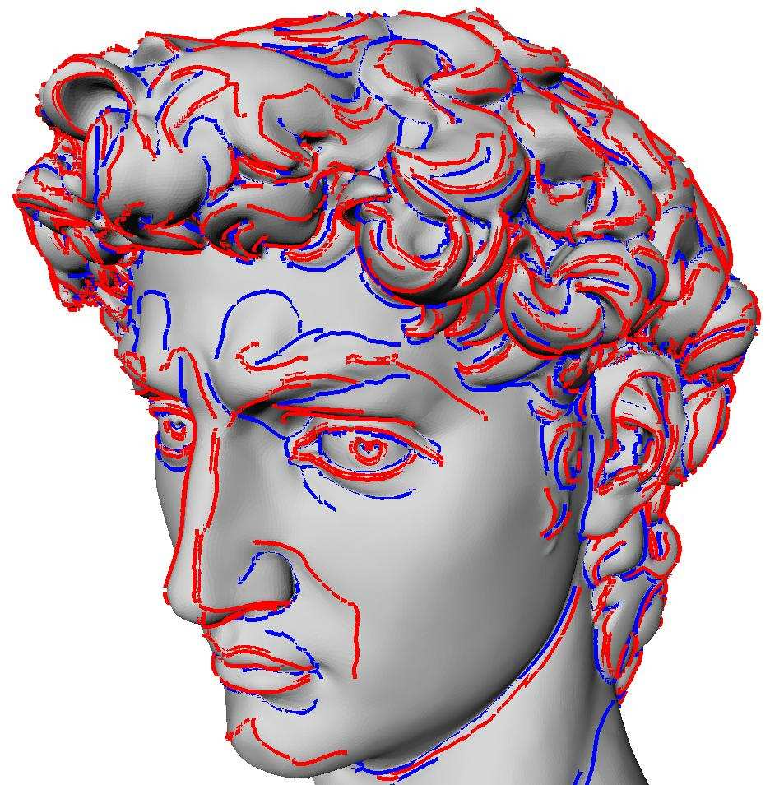
\includegraphics[width=.5\linewidth]{Ridges_3/david_crest}}
\end{ccTexOnly}

\label{david-crest}
\begin{ccHtmlOnly}
<CENTER> <img border=0 src="./david_crest.jpg" width=400>
</CENTER>
\end{ccHtmlOnly}
\caption{Crest ridges on the David, model provided by the Digital Michelangelo Project.}
\end{figure}

This chapter describes the \cgal\ package for the approximating the
ridges and umbilics of a smooth surface discretized by a triangle
mesh.  Given a smooth surface, a ridge is a curve along which one of
the principal curvatures has an extremum along its curvature line. An
umbilic is a point at which both principal curvatures are
equal. Ridges define a singular curve, i.e., a self-intersecting
curve, and umbilics are special points on this curve. Ridges are
curves of {\em extremal} curvature and therefore encode important
informations used in segmentation, registration, matching and surface
analysis.  Based on the results of the article
\cite{cgal:cp-tdare-05}, we propose algorithms to identify and extract
different parts of this singular ridge curve as well as umbilics on a
surface given as a triangulated surface mesh. Differential quantities
associated to the mesh vertices are assumed to be given for these
algorithms; such quantities may be computed by the package {\em
Estimation of Local Differential Properties of Sampled Surfaces via
Polynomial Fitting}.

Note that this package needs the third party library \ccThirdPartyEigen for linear algebra operations.

\subsection{Overview}
%%%%%%%%%%%%%%%%%%%%%%

Section \ref{smooth} presents the basics of the theory of ridges and
umbilics on smooth surfaces. Sections \ref{ridge-mesh} and
\ref{umbilic-mesh} present algorithms for  approximating the ridges and
umbilics (of a smooth surface) from a triangle mesh. Section
\ref{soft} gives the package specifications, while example calls to
functions of the package are provided in Section~\ref{examples}.


\section{Ridges and Umbilics of a Smooth Surface\label{smooth}}
%%%%%%%%%%%%%%%%%%%%%%%%%%%%%%%%%%%%%%%

For a detailed introduction to ridges and related topics, the reader
may consult 
\cite{cgal:hgygm-ttdpf-99,cgal:p-gd-01}, as well as
the following survey article \cite{cgal:cp-ssulc-05}.
%%
In the sequel, we just introduce the basic notions so as to explain
our algorithms.  Consider a smooth embedded surface, and denote $k_1$
and $k_2$ the principal curvatures, with $k_1\geq k_2$. Umbilics are
the points where $k_1=k_2$.  For any non umbilical point, the
corresponding principal directions of curvature are well defined, and
we denote them $d_1$ and $d_2$.
%%
In local coordinates, we denote $\langle , \rangle$ the inner product
induced by the ambient Euclidean space, and $dk_1$, $dk_2$ the
gradients of the principal curvatures. Ridges, illustrated in Figure
\ref{ellipsoid-ridges} for the standard ellipsoid, are defined by:

\begin{definition}
\label{def:ridge-extrema}
A non umbilical point is called
\begin{itemize}
\item
a max ridge point, if the {\em extremality coefficient} $b_0=\langle
dk_1,d_1 \rangle$ vanishes, i.e. $b_0=0$.

\item a min ridge point, if the {\em extremality coefficient}
  $b_3=\langle dk_2,d_2 \rangle$ vanishes, i.e. $b_3=0$
  \footnote{Notations $b_0, b_3$ comes from Equation~\ref{eq:monge} }.
\end{itemize}
\end{definition}

%%
The previous characterization of ridges involves third-order
differential properties. Using fourth-order differential quantities, a
ridge point can further be qualified as {\em elliptic} if it
corresponds to a maximum of $k_1$ or a minimum of $k_2$, or {\em
hyperbolic} otherwise. Hence we end up with four types of ridges, namely:
 \ccc{MAX_ELLIPTIC_RIDGE}, \ccc{MAX_HYPERBOLIC_RIDGE}, \ccc{MIN_ELLIPTIC_RIDGE},
\ccc{MIN_HYPERBOLIC_RIDGE}, which are illustrated in  Figure~\ref{ellipsoid-ridges}.
%%
Also of interest are the {\em crest lines}, a crest line being an
elliptic ridge which is a maximum of $\max(|k_1|,|k_2|)$. Crest lines
form a subset of elliptic ridges, and can be seen as the visually most
salient curves on a surface.
%%
Hence we provide the two additional ridge types
\ccc{MAX_CREST_RIDGE} and \ccc{MIN_CREST_RIDGE}, which are illustrated  in
Figure~\ref{david-crest}.

\begin{figure}[!ht]
\begin{ccTexOnly}
\centerline{
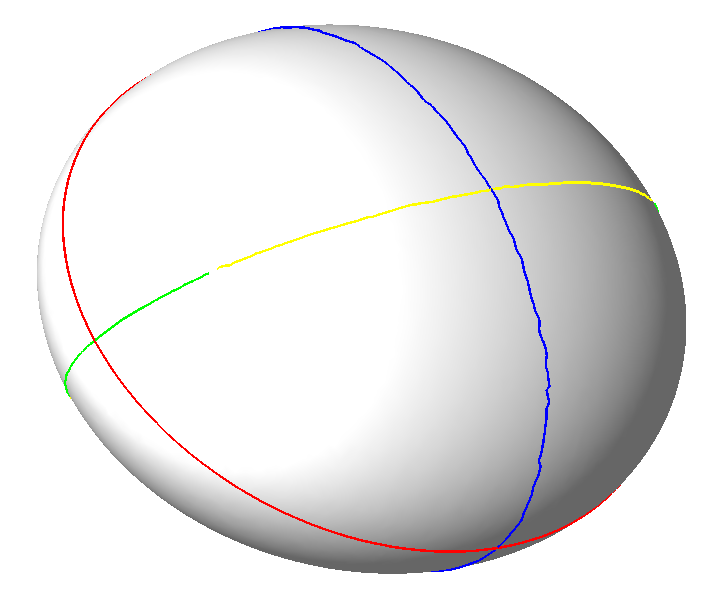
\includegraphics[width=.5\linewidth]{Ridges_3/ellipsoid_ridges}}
\end{ccTexOnly}

\begin{ccHtmlOnly}
<CENTER> <img border=0 src="./ellipsoid_ridges.png" width=400>
</CENTER>
\end{ccHtmlOnly}
\caption{Ridges on the ellipsoid, normals pointing outward.  Color
  coding: \ccc{MAX_ELLIPTIC_RIDGE} are blue,
  \ccc{MAX_HYPERBOLIC_RIDGE} are green, \ccc{MIN_ELLIPTIC_RIDGE} are
  red and \ccc{MIN_HYPERBOLIC_RIDGE} are yellow. The red line is also
  the \ccc{MIN_CREST_RIDGE} and this is the only crest ridge of the
  ellipsoid.}
\label{ellipsoid-ridges}
\end{figure}

At any point of the surface which is not an umbilic, principal
directions $d_1, d_2$ are well defined, and these (non oriented)
directions together with the normal vector $n$ define two direct
orthonormal frames. If $v_1$ is a unit vector of direction $d_1$ then
there exists a unique unit vector $v_2$ so that $(v_1,v_2,n)$ is
direct, that is has the same orientation as the canonical basis of the
ambient $3d$ space (and the other possible frame is $(-v_1,-v_2,n)$). In the
coordinate systems $(v_1,v_2,n)$, the surface has the following
canonical form, known as the Monge form~:
%
\begin{eqnarray}
\label{eq:monge}
z(x,y) =  & \frac{1}{2}(k_1x^2 + k_2y^2)+
	\frac{1}{6}(b_0x^3+3b_1x^2y+3b_2xy^2+b_3y^3) \\
  &  +\frac{1}{24}(c_0x^4+4c_1x^3y+6c_2x^2y^2+4c_3xy^3+c_4y^4) + \hot
\end{eqnarray}

\noindent The Taylor expansion of $k_1$ (resp. $k_2$) along the max
(resp. min) curvature line going through the origin and parameterized
by $x$ (resp. $y$) are:
\begin{equation}
\label{eq:taylor_along_line}
k_1(x) = k_1 + b_0x + \frac{P_1}{2(k_1-k_2)}x^2 +\hot , \quad \quad \quad
P_1= 3b_1^2+(k_1-k_2)(c_0-3k_1^3).
\end{equation}
%
\begin{equation}
\label{eq:taylor_along_red_line}
k_2(y) = k_2 + b_3y + \frac{P_2}{2(k_2-k_1)}y^2 +\hot , \quad \quad \quad
P_2= 3b_2^2+(k_2-k_1)(c_4-3k_2^3).
\end{equation}

\noindent Notice also that switching from one to the other of the two
afore-mentioned coordinate systems reverts the sign of all the odd
coefficients on the Monge form of the surface.
\medskip

Hence ridge types are characterized by 
\begin{itemize}
\item max ridge if $b_0=0$
\item \ccc{MAX_ELLIPTIC_RIDGE} if $b_0=0$ and $P_1<0$
\item \ccc{MAX_HYPERBOLIC_RIDGE} if $b_0=0$ and $P_1>0$
\item min ridge if $b_3=0$
\item \ccc{MIN_ELLIPTIC_RIDGE} if $b_3=0$ and $P_2<0$
\item \ccc{MIN_HYPERBOLIC_RIDGE} if $b_3=0$ and $P_2>0$
\item \ccc{MAX_CREST_RIDGE} if $b_0=0$ and $P_1<0$ and $|k_1|>|k_2|$
\item \ccc{MIN_CREST_RIDGE} if $b_3=0$ and $P_2<0$ and $|k_2|>|k_1|$
\end{itemize}


As illustrated in Figures~\ref{index_umbilic} and \ref{umbilics}, the
patterns made by curvature lines around an umbilic can be
characterized using the notion of an {\em index} associated to the
principal directions --- see also \cite{cgal:cp-ssulc-05}.
%%
As depicted in Figure~\ref{index_umbilic}, consider a small circuit $C$ around the
umbilic, and a point $p \in C$. Starting from an initial orientation
$u$ of a tangent vector to the curvature line through point $p$,
propagate {\em by continuity} this orientation around the circuit.  The
index is defined by the angle swept by $u$ around this revolution,
normalized by $2\pi$. In our example, the index is thus 1/2.

If the index of the principal direction field is $1/2$
then it is called a
\ccc{ELLIPTIC_UMBILIC}, if it is $-1/2$ it is called a \ccc{HYPERBOLIC_UMBILIC}.
 Otherwise the umbilic is qualified
\ccc{NON_GENERIC_UMBILIC}.


\begin{figure}[!ht]
\begin{ccTexOnly}
\centerline{
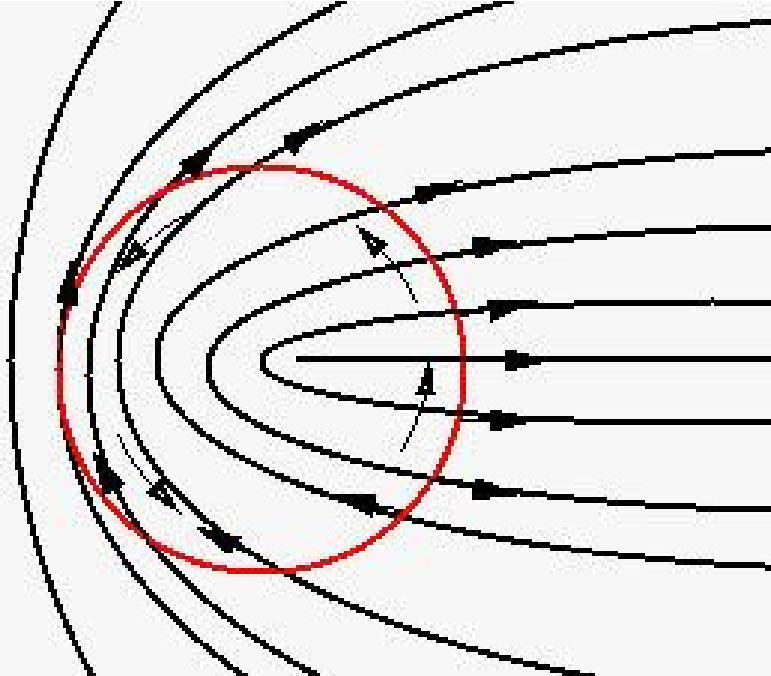
\includegraphics[width=.5\linewidth]{Ridges_3/index_umbilic}}
\end{ccTexOnly}

\begin{ccHtmlOnly}
<CENTER> <img border=0 src="./index_umbilic.png" width=200>
</CENTER>
\end{ccHtmlOnly}
\caption{Index $1/2$ umbilic or elliptic umbilic.}
\label{index_umbilic}
\end{figure}


\begin{figure}[!ht]
\begin{ccTexOnly}
\centerline{
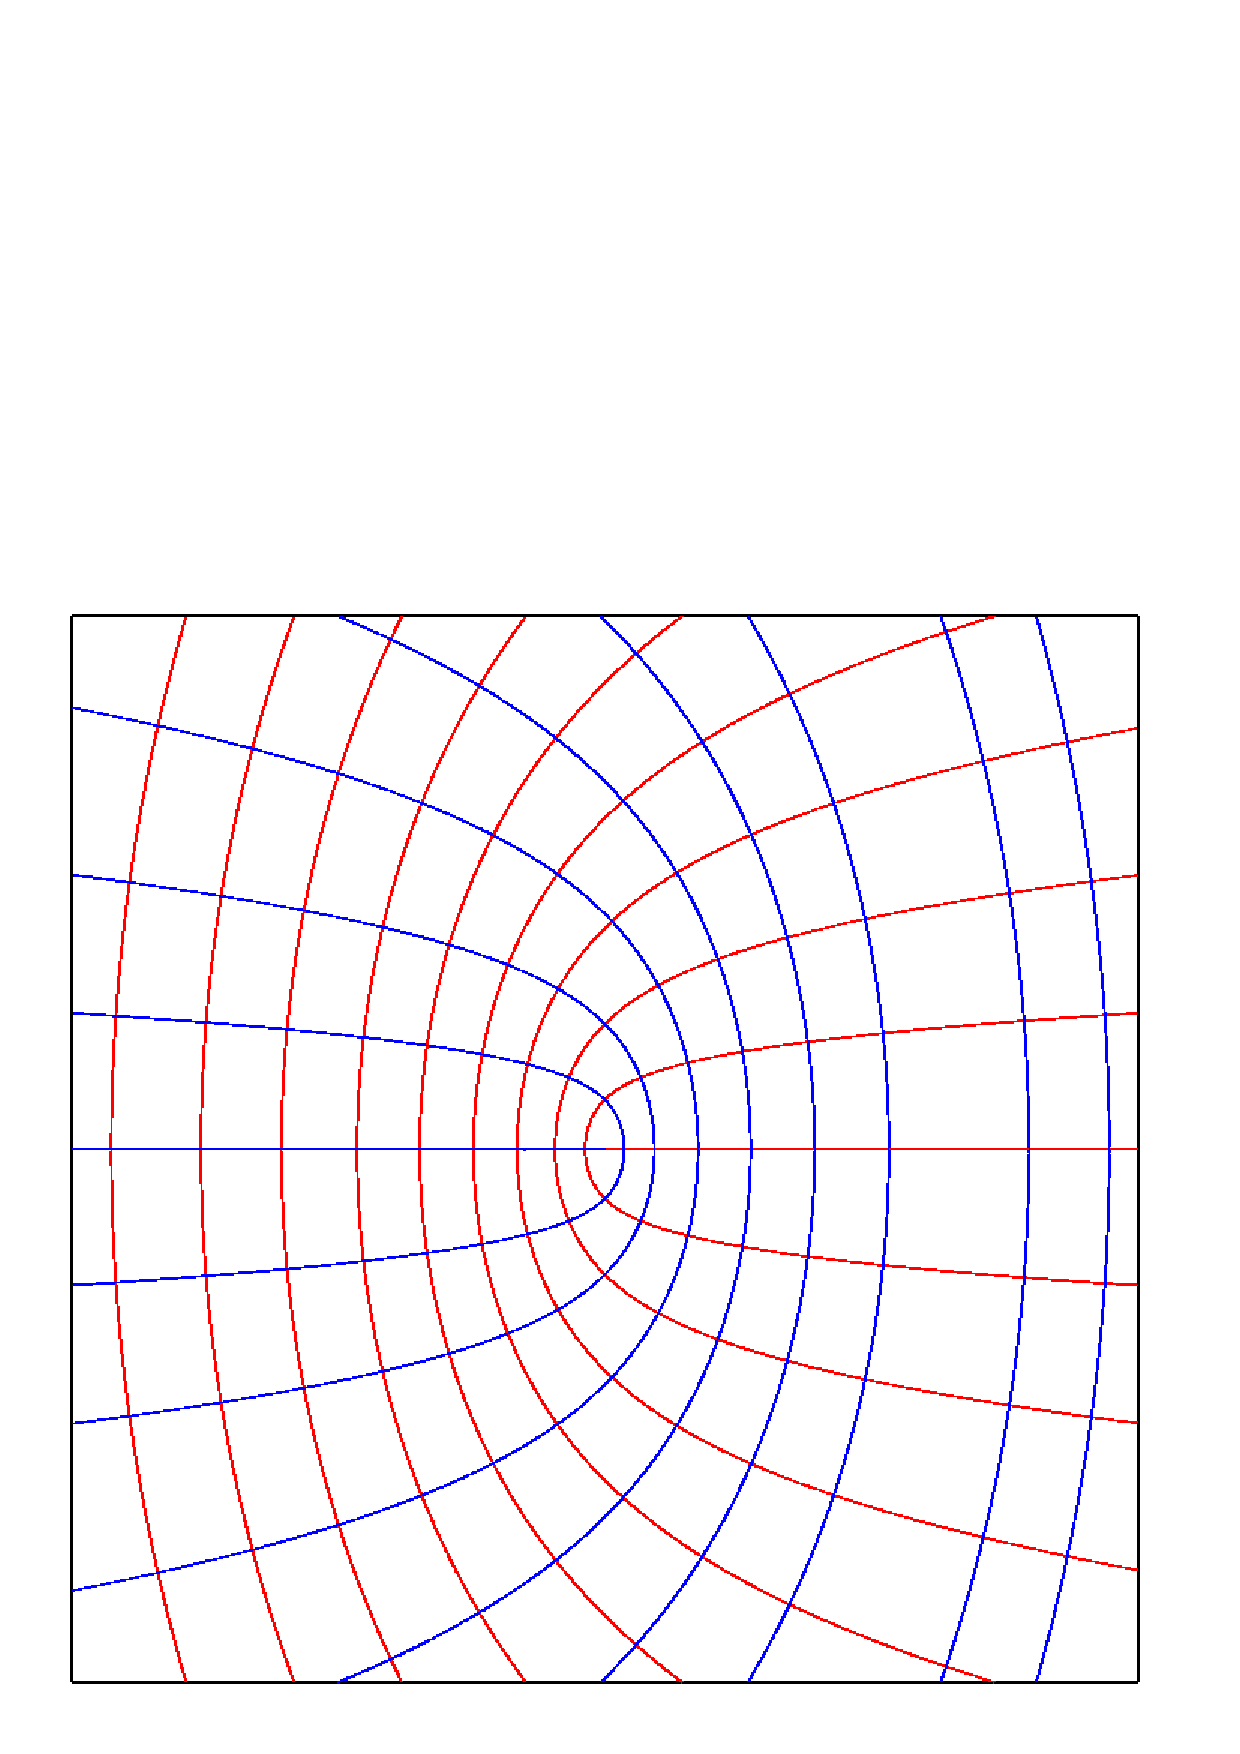
\includegraphics[width=.5\linewidth]{Ridges_3/lemon}
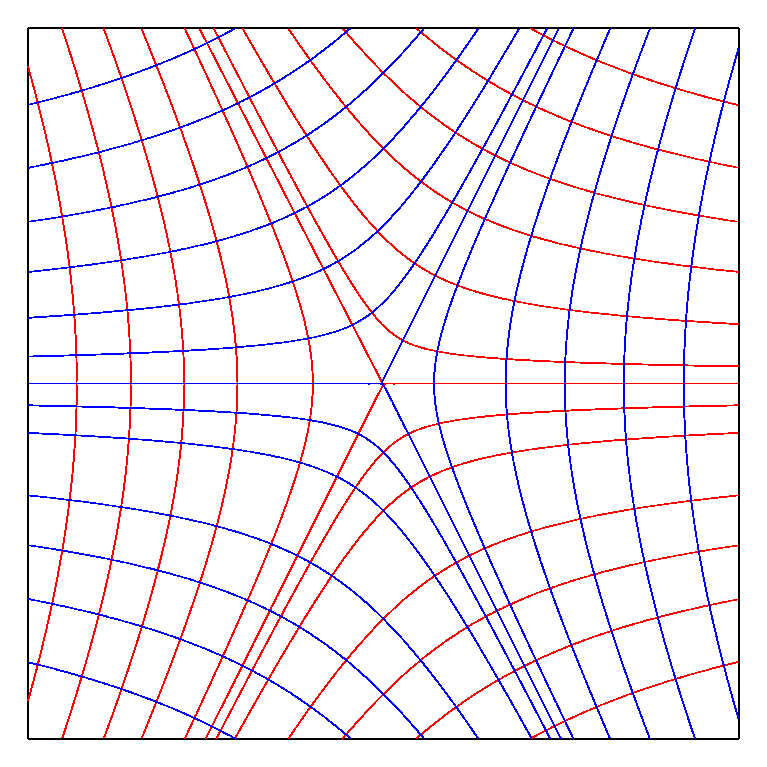
\includegraphics[width=.5\linewidth]{Ridges_3/star}}
\end{ccTexOnly}

\begin{ccHtmlOnly}
<CENTER> <img border=0 src="./lemon.png" width=300>
 <img border=0 src="./star.png" width=300>
</CENTER>
\end{ccHtmlOnly}
\caption{Elliptic and hyperbolic umbilics.}
\label{umbilics}
\end{figure}



\section{Approximating  Ridges on Triangulated Surface Meshes}
%%%%%%%%%%%%%%%%%%%%%%%%%%%%%%%%%
\label{ridge-mesh}

Our method aims at reporting ridges as polygonal lines living on the
mesh. It assumes differential quantities are available for each vertex
of the mesh (principal curvatures and directions together with third
order quantities $b_0, b_3$ and optionally fourth order quantities
$P_1, P_2$). These differential quantities may be computed for the
smooth surface the mesh is inscribed in (analytically or using
approximation methods), or may be estimated for a mesh given without
reference to an underlying smooth surface. Although the ridge
approximation algorithm is the same in both cases, one cannot ambition
to ask for the same certificates.  This distinction calls for the
notion of {\em compliant} mesh.


\paragraph{Compliant meshes.}
Ridges of a smooth surface are points with prescribed differential
properties, and reporting them from a mesh inscribed in the surface
requires delicate hypothesis on the geometry of that mesh so as to get
a certified result. In this paragraph, we assume the mesh provided
complies with a number of hypothesis, which guarantee the topology of
the ridges reported matches that of the ridges on the smooth
surface. To summarize things, a compliant mesh is a mesh dense enough
so that (i)\ umbilics are properly isolated (ii)\ ridges running next
to one another are also properly separated.
%%
See \cite{cgal:cp-tdare-05} for a detailed discussion of {\em
compliant} meshes.  \medskip

As 0-level set of the extremality coefficients $b_0$ and $b_3$, ridges
are extracted by a marching triangles algorithm.\footnote{A marching
triangles algorithm is similar to a 2d marching cubes algorithm (or
marching rectangles algorithm), except that a one-manifold is
reported on a two-manifold tessellated by triangles.}

%% instead of  rectangles.}.
%%
%%on the surface.  
%%
As the signs of these extremality coefficients depend on the
orientation of the principal directions, we expect both extremalities
and vectors orienting the principal direction to be given at each
point vertex of the mesh. Except in the neighborhood of umbilics, if
the mesh is dense enough, a coherent orientation of principal
directions at both endpoints of an edge is chosen such that the angle
between the two vectors is acute. This rule, the {\em acute rule}, is
precisely analyzed in \cite{cgal:cp-tdare-05}.
%%
Moreover, we only seek ridges in triangles for which one can find an
orientation of its three vertices such that the three edges are
coherently oriented by the acute rule. Such triangles are called
{\em regular}. This said, two remarks are in order.

\noindent {\em ---Regular triangles and ridge segments.}
A regular triangle has 0 or 2 edges crossed by a max (resp. min)
ridge, which is tantamount to a sign change of $b_0$ (resp. $b_3$)
along the corresponding edges. In the latter case, we say that the
triangle contains a ridge segment.
%%
Two methods are provided to compute its type, be it elliptic or
hyperbolic. First, if fourth order differential quantities are
provided, one can use the $P_1$ ($P_2$) values of Equations
\ref{eq:taylor_along_line} (\ref{eq:taylor_along_red_line}) for a
max (min) ridge. The value of $P_i$ for a ridge segment is defined as
the mean value of the $P_i$ values of the two crossing points on edges
(while the value at a crossing point on an edge is the $b_i$-weighted
mean value of the values at endpoints).
%%
Alternatively, if third order differential quantities only are
available, one may use the geometric method developed in
\cite{cgal:cp-tdare-05}.


Using the notion of ridge segment, a \ccc{Ridge_line} is defined as a
maximal connected sequence of ridge segments of the same type and connected
together.  Notice that the topology of a \ccc{Ridge_line} is either
that of an interval or a circle.

\noindent {\em ---Non-regular triangles.}  In the neighborhood of umbilics,
triangle are less likely to be regular and the detection of ridges
cannot be relevant by this method.  This is why we propose another
method to detect umbilics independently.

\paragraph{Non compliant meshes: filtering ridges on {\em
strength} and {\em sharpness}.}
%%
For real world applications dealing with coarse meshes, or meshes
featuring degenerate regions or sharp features, or meshes conveying
some amount of noise, the {\em compliance} hypothesis
\cite{cgal:cp-tdare-05} cannot be met. In that case, it still makes
sense to seek loci of points featuring extremality of estimated
principal curvatures, but the ridges reported may require
filtering. For example, if the principal curvatures are constant
---which is the case on a plane or a cylinder, then all points are
ridge points. In this context, an appealing notion is that of {\em
sharp} ridge or {\em prominent} ridge. Since ridges are witnessed by
zero crossings of $b_0$ and $b_3$, one can expect erroneous detections
as long as these coefficients remain small. In order to select the
most prominent ridge points, we focus on points where the variation of
the curvature is fast along the curvature line.  One can observe that,
at a ridge point, according to  Equation
\ref{eq:taylor_along_line}, the second derivative of $k_1$ along its
curvature line satisfies $k_1^{''}(0) = P_1/(k_1-k_2)$.  Using this
observation, one can define the {\em sharpness of a ridge} as the
integral of the absolute value of $P_1/(k_1-k_2)$ along the ridge. As
the second derivative of the curvature is homogeneous to the inverse
of the cube of a length, the sharpness is homogeneous to the inverse
of the square of a length. Multiplying the sharpness by the square of
the model size gives a threshold and an associated sharpness-filter
which are scale independent. Another filtering is also available with
the {\em strength } which is the integral of the curvature along the
ridge line
\cite{cgal:ybs-rvlmi-04}.





\section{Approximating Umbilics on Triangulated Surface Meshes}
%%%%%%%%%%%%%%%%%%%%%%%%%%%%%%%%%
\label{umbilic-mesh}

The method aims at identifying some vertices of a mesh as umbilics. It
assumes principal curvatures and directions are given at each vertex
on the mesh.
%The detection of umbilics is based upon a two stages methods, which
%both require finding a topological disk around the umbilic.
%
%The method combines a minimization and an index computation (of the
%principal direction field) on the neighborhood of each vertex of $T$.

\paragraph{Algorithm.}
Assume each vertex $v$ of the mesh comes with a patch (a topological
disk) around it. Checking whether vertex $v$ is an umbilic is a two
stages process, which are respectively concerned with the variation
of the function $k_1-k_2$ over the patch, and the index of the vertex
computed from the boundary of the patch. More precisely, vertex $v$ is
declared to be an umbilic if the following two conditions are met:
%%
\begin{itemize}
\item
the function $k_1-k_2$ has its minimum at $v$ amongst all the
vertices of the patch;
\item
the deviation $\delta$ of any principal direction along the patch
boundary, traversed counter-clock-wise (CCW), has prescribed
properties:
%%
\begin{itemize}
\item
$\delta \in ]\pi/2,3\pi/2[$, then the umbilic is called elliptic,
\item
$\delta \in ]-3\pi/2,-\pi/2[$, then the umbilic is called a hyperbolic,
\item
otherwise the umbilic is called non-generic.
\end{itemize}
\end{itemize}

\paragraph{Finding patches around vertices.}
Given a vertex $v$ and a parameter $t$, we aim at defining a
collection of triangles around $v$ so that (i) this collection defines
a topological disk on the triangulation $T$ and (ii) its size depends
on $t$. First we collect the 1-ring triangles. We define the size $s$
of this 1-ring patch as the (Euclidean) distance from $v$ to its
farthest 1-ring vertex neighbor. We then collect recursively adjacent
triangles so that the patch remains a topological disk and such that
these triangles are at distance less than $s\times t$. Parameter $t$
is the only parameter of the algorithm.

\paragraph{Umbilical patches versus ridges.} On a generic surface,
generic umbilics are traversed by one or three ridges. For compliant
meshes, an umbilic can thus be connected to the ridge points located
on the boundary of its patch. This functionality is not provided, and
the interested reader is referred to \cite{cgal:cp-tdare-05} for more
details.

%%%%%%%%%%%%%%%%%%%%%%%
\section{Software Design}
%%%%%%%%%%%%%%%%%%%%%%%
\label{soft}

All classes of this package are templated by the parameter
\ccc{TriangulatedSurfaceMesh}, which defines the type of the mesh to which the
approximation algorithms operate.

The differential quantities are provided at vertices of this mesh via
property maps, a concept commonly used in the Boost library. Scalar
data (curvatures and their derivatives) are provided via
\ccc{Vertex2FTPropertyMap} concepts, while  $3d$ vector data (principal
directions of curvatures) are provided via
\ccc{Vertex2VectorPropertyMap} concepts. 
The rationale for introducing these concepts is that properties are
used independently from the way they are stored. This enables the user
to store them {\em internally} in extended vertices or {\em externally}
with maps. We provide a class
\ccc{Vertex2Data_Property_Map_with_std_map} to adapt \ccc{std::map} with 
a \ccc{boost::associative_property_map} to model these concepts.


Output of ridges or umbilics are provided via output iterator.

Approximation of ridges and umbilics are performed by two independent
classes, which we now further describe.

\subsection{Ridge Approximation}
%%%%%%%%%%%%%%%


The main class is
\ccc{Ridge_approximation<TriangulatedSurfaceMesh,Vertex2FTPropertyMap,Vertex2VectorPropertyMap>}.
Its construction requires the mesh and the property maps defining the
differential quantities for principal curvatures $k_1$ and $k_2$, the
third order extremalities $b_0$ and $b_3$, the principal directions of
curvature $d_1$ and $d_2$, and the fourth order quantities $P_1$ and
$P_2$ if the tagging of ridges as elliptic or hyperbolic is to be done using
the polynomials $P_1$ and $P_2$.


Three functions (provided as members and also as global functions)
enable the computation of different types of ridges~:
\begin{itemize}
\item \ccc{compute_max_ridges} (resp. \ccc{compute_min_ridges})
  outputs ridges of types \ccc{MAX_ELLIPTIC_RIDGE} and
  \ccc{MAX_HYPERBOLIC_RIDGE} (resp. \ccc{MIN_ELLIPTIC_RIDGE} and
  \ccc{MIN_HYPERBOLIC_RIDGE}).
\item \ccc{compute_crest_ridges} outputs ridges of types
  \ccc{MAX_CREST_RIDGE} and \ccc{MIN_CREST_RIDGE}.
\end{itemize}

These functions allows the user to specify how the elliptic/hyperbolic
tagging is carried out.
%%
Notice the rationale for the choice of these three functions is
simple: each computation needs a single pass over the triangles of the
mesh. This should be clear for the min and max ridges. For crests,
just notice max and min crests cannot intersect over a triangle.
\medskip

The ridge lines are stored in
\ccc{Ridge_line} objects and output through an iterator. 
Each ridge line is represented as a list of halfedges of the mesh it
crosses with a scalar defining the barycentric coordinate of the
crossing point with respect to the half-egde endpoints. Each ridge
line comes with its type \ccc{Ridge_type}, its strength and sharpness.

If one chooses to use only third order quantities, the quantities
$P_i$ do not have to be defined. Then the sharpness will not be
defined.

\subsection{Umbilic Approximation}
%%%%%%%%%%%%%%%%%%%%%
The main class is
\ccc{Umbilic_approximation<TriangulatedSurfaceMesh,Vertex2FTPropertyMap,Vertex2VectorPropertyMap>}.
Its construction requires the mesh and the property maps defining the
differential quantities for principal curvatures $k_1$ and $k_2$, and
the principal directions of curvature $d_1$ and $d_2$.  The member
function \ccc{compute} (or the global function \ccc{compute_umbilics})
has a parameter to define the size of the neighborhood of the umbilic.

Umbilics are stored in \ccc{Umbilic} objects, they come with their
type : \ccc{ELLIPTIC_UMBILIC}, \ccc{HYPERBOLIC_UMBILIC} or
\ccc{NON_GENERIC_UMBILIC}; the vertex of the mesh they are associated
to and the list of half-edges representing the contour of the
neighborhood.

\subsection{Models for the Property Map Concepts}
%%%%%%%%%%%%%%%%%%%%%%%%%%%%%%%%%%%%%%%%%%%%%%%%%%%%%%%%%%%%%%%%%%%%%%%%%%%%
The class
\ccc{Vertex2Data_Property_Map_with_std_map<TriangulatedSurfaceMesh>}
enables the definition of models for the concepts
\ccc{Vertex2FTPropertyMap} and
\ccc{Vertex2VectorPropertyMap} 
using \ccc{std::maps} and \ccc{boost::associative_property_map}.


\section{Examples}

%%%%%%%%%%%%%%%%%%%%%%%%%%%%%%%%%%%%%%%%%%%%%%%%%%%%%%%%%%%%%%%%%%%%%%%%%%%%
\label{examples}

\subsection{Example program}
The following program computes ridges and umbilics from an off
file.\footnote{Model data may be downloaded via
  ftp://ftp.mpi-sb.mpg.de/pub/outgoing/CGAL/Ridges\_3\_datafiles.tgz .
  The mechanical part model has been provided courtesy of Dassault
  System to produce Figure~\ref{fig:mechanical_crest_filtered-intro},
  due to copyright issues the available model is not the same, it is
  provided by the AIM@SHAPE Shape Repository.} It uses the Jet fitting package to estimate the differential
quantities. 
%introspect-qt and the demo rep not in the public release%%% 
%The output file contains data to be visualized with the
%demo program introspect-qt.  
The default output file gives rough data for visualization purpose, a
verbose output file may also be asked for.  Parameters are
\begin{itemize}
\item
$d$, the degree of the jet for the \ccc{Monge_via_jet_fitting} class, $d$
must be greater or equal to 3 which is the default value;
\item
$m$, the degree of the Monge representation for the
\ccc{Monge_via_jet_fitting} class, $m$ must be 3 (the default value) or
4 and smaller than $d$;
\item
$a$, the number of rings of neighbors collected for the
\ccc{Monge_via_jet_fitting} class, in addition the number of vertices
collected must be greater than $Nd:=(d+1)(d+2)/2$ to make the
approximation possible. $a$ may be an integer greater than 1, the value
0 (which is the default) means that the minimum number of rings is
collected to make the approximation possible. (Alternatively option $p$
allows the specification of a constant number of neighbors);
\item
$t$, the \ccc{CGAL::Ridge_order} for the distinction between elliptic and
hyperbolic ridges, $t$ is 3 (default) or 4;
\item
$u$, the parameter for umbilic patch size, $u \geq 1$ (default is 1).
\end{itemize}

\begin{ccExampleCode} 
#include <CGAL/Ridges.h> 
#include <CGAL/Umbilics.h>

//this is an enriched Polyhedron with facets' normal
#include "PolyhedralSurf.h"

typedef PolyhedralSurf::Traits          Kernel;
typedef Kernel::FT                      FT;
typedef Kernel::Point_3                 Point_3;
typedef Kernel::Vector_3                Vector_3;

typedef PolyhedralSurf::Vertex_const_handle   Vertex_const_handle;
typedef PolyhedralSurf::Vertex_const_iterator Vertex_const_iterator;
    
typedef CGAL::Vertex2Data_Property_Map_with_std_map<PolyhedralSurf> Vertex2Data_Property_Map_with_std_map;
typedef Vertex2Data_Property_Map_with_std_map::Vertex2FT_map Vertex2FT_map;
typedef Vertex2Data_Property_Map_with_std_map::Vertex2Vector_map Vertex2Vector_map;
typedef Vertex2Data_Property_Map_with_std_map::Vertex2FT_property_map Vertex2FT_property_map;
typedef Vertex2Data_Property_Map_with_std_map::Vertex2Vector_property_map Vertex2Vector_property_map;

//RIDGES
typedef CGAL::Ridge_line<PolyhedralSurf> Ridge_line;
typedef CGAL::Ridge_approximation < PolyhedralSurf,
				    back_insert_iterator< std::vector<Ridge_line*> >,
				    Vertex2FT_property_map,
				    Vertex2Vector_property_map > Ridge_approximation;
//UMBILICS
typedef CGAL::Umbilic<PolyhedralSurf> Umbilic;
typedef CGAL::Umbilic_approximation < PolyhedralSurf,
				      back_insert_iterator< std::vector<Umbilic*> >, 
				      Vertex2FT_property_map, 
				      Vertex2Vector_property_map > Umbilic_approximation;

//create property maps
Vertex2FT_map vertex2k1_map, vertex2k2_map, 
  vertex2b0_map, vertex2b3_map, 
  vertex2P1_map, vertex2P2_map;
Vertex2Vector_map vertex2d1_map, vertex2d2_map;

Vertex2FT_property_map vertex2k1_pm(vertex2k1_map), vertex2k2_pm(vertex2k2_map), 
  vertex2b0_pm(vertex2b0_map), vertex2b3_pm(vertex2b3_map), 
  vertex2P1_pm(vertex2P1_map), vertex2P2_pm(vertex2P2_map);
Vertex2Vector_property_map vertex2d1_pm(vertex2d1_map), vertex2d2_pm(vertex2d2_map);

int main(int argc, char *argv[])
{  
  //compute differential quantities with the jet fitting package
	...
  //initialize the property maps
	...
   //---------------------------------------------------------------------------
  //Ridges
  //--------------------------------------------------------------------------
  Ridge_approximation ridge_approximation(P, 
					  vertex2k1_pm, vertex2k2_pm,
					  vertex2b0_pm, vertex2b3_pm,
					  vertex2P1_pm, vertex2P2_pm,
					  vertex2d1_pm, vertex2d2_pm);
  std::vector<Ridge_line*> ridge_lines;
  back_insert_iterator<std::vector<Ridge_line*> > ii(ridge_lines);
  
  //Find MAX_RIDGE, MIN_RIDGE, CREST or all ridges
  ridge_approximation.compute_max_ridges(ii, tag_order);  
  ridge_approximation.compute_min_ridges(ii, tag_order);  
  ridge_approximation.compute_crest_ridges(ii, tag_order);  

  //---------------------------------------------------------------------------
  // UMBILICS
  //--------------------------------------------------------------------------
  Umbilic_approximation umbilic_approximation(P, 
					      vertex2k1_pm, vertex2k2_pm,
					      vertex2d1_pm, vertex2d2_pm);
  std::vector<Umbilic*> umbilics;
  back_insert_iterator<std::vector<Umbilic*> > umb_it(umbilics);
  umbilic_approximation.compute(umb_it, umb_size);
 }
\end{ccExampleCode}

\subsection{Example: Ridges and Umbilics  on an Ellipsoid}

For Figure\ref{ellipsoid-ridges-example}, the data have been computed as follows:
%%
\begin{ccExampleCode}
./Compute_Ridges_Umbilics -f data/ellipsoid_u_0.02.off -d 4 -m 4 -a 3 -t 3
\end{ccExampleCode}
% and the visualization with 
% \begin{ccExampleCode}
%  ../../demo/Ridges_3/introspect-qt data/ellipsoid_u_0.02.off data/data_ellipsoid_u_0.02.offRIDGES-d4-m4-t4-a3-p0.4ogl.txt 0 0
% \end{ccExampleCode} 
In addition, the four elliptic umbilics are detected, the standard output being
\begin{ccExampleCode}
nb of umbilics 4
Umbilic at location (-0.80899 0.00426003 0.293896) of type elliptic
Umbilic at location (-0.811197 0.0122098 -0.292259) of type elliptic
Umbilic at location (0.808372 -0.00551307 -0.29431) of type elliptic
Umbilic at location (0.81413 0.0018689 0.290339) of type elliptic
\end{ccExampleCode}


\begin{figure}[!ht]
\begin{ccTexOnly}
\centerline{
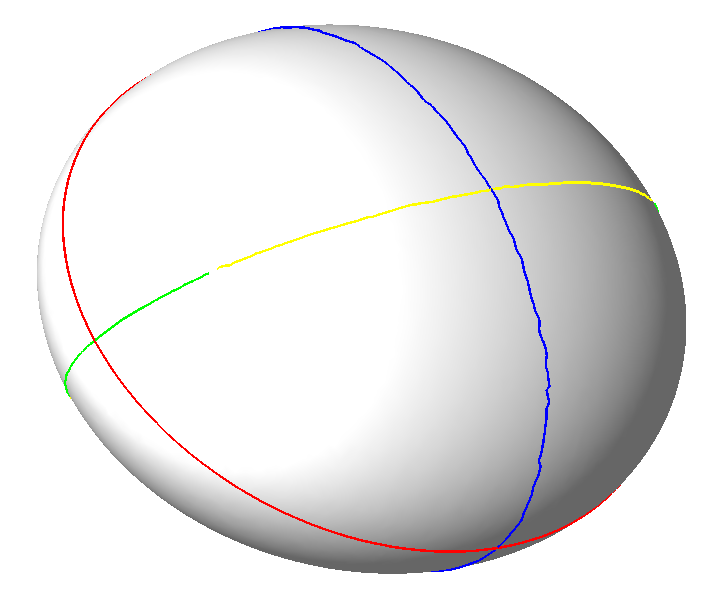
\includegraphics[width=.5\linewidth]{Ridges_3/ellipsoid_ridges}}
\end{ccTexOnly}

\begin{ccHtmlOnly}
<CENTER> <img border=0 src="./ellipsoid_ridges.png" width=400>
</CENTER>
\end{ccHtmlOnly}
\caption{Ridges on the ellipsoid, normals pointing outward.
 Color coding~: \ccc{MAX_ELLIPTIC_RIDGE} are blue,
\ccc{MAX_HYPERBOLIC_RIDGE} are green, \ccc{MIN_ELLIPTIC_RIDGE} are red and 
\ccc{MIN_HYPERBOLIC_RIDGE} are yellow. }
\label{ellipsoid-ridges-example}
\end{figure}

\subsection{Example: Filtering of Crest Ridges on a Mechanical Par}

Figure~\ref{fig:mechanical_crest_filtered-intro} illustrates the filtering 
of crest ridges on a mechanical model, and has been computed as follows:
%%
\begin{ccExampleCode}
./Compute_Ridges_Umbilics -f data/mecanic.off -d 4 -m 4 -a 4 -t 4
\end{ccExampleCode}
% The last parameters of the visualization program of the demo are
% threshold for the strength and the sharpness. This enables the three
% different images to be produced with the same data.

\begin{figure}[htb] 
\begin{ccTexOnly}
\centerline{ 
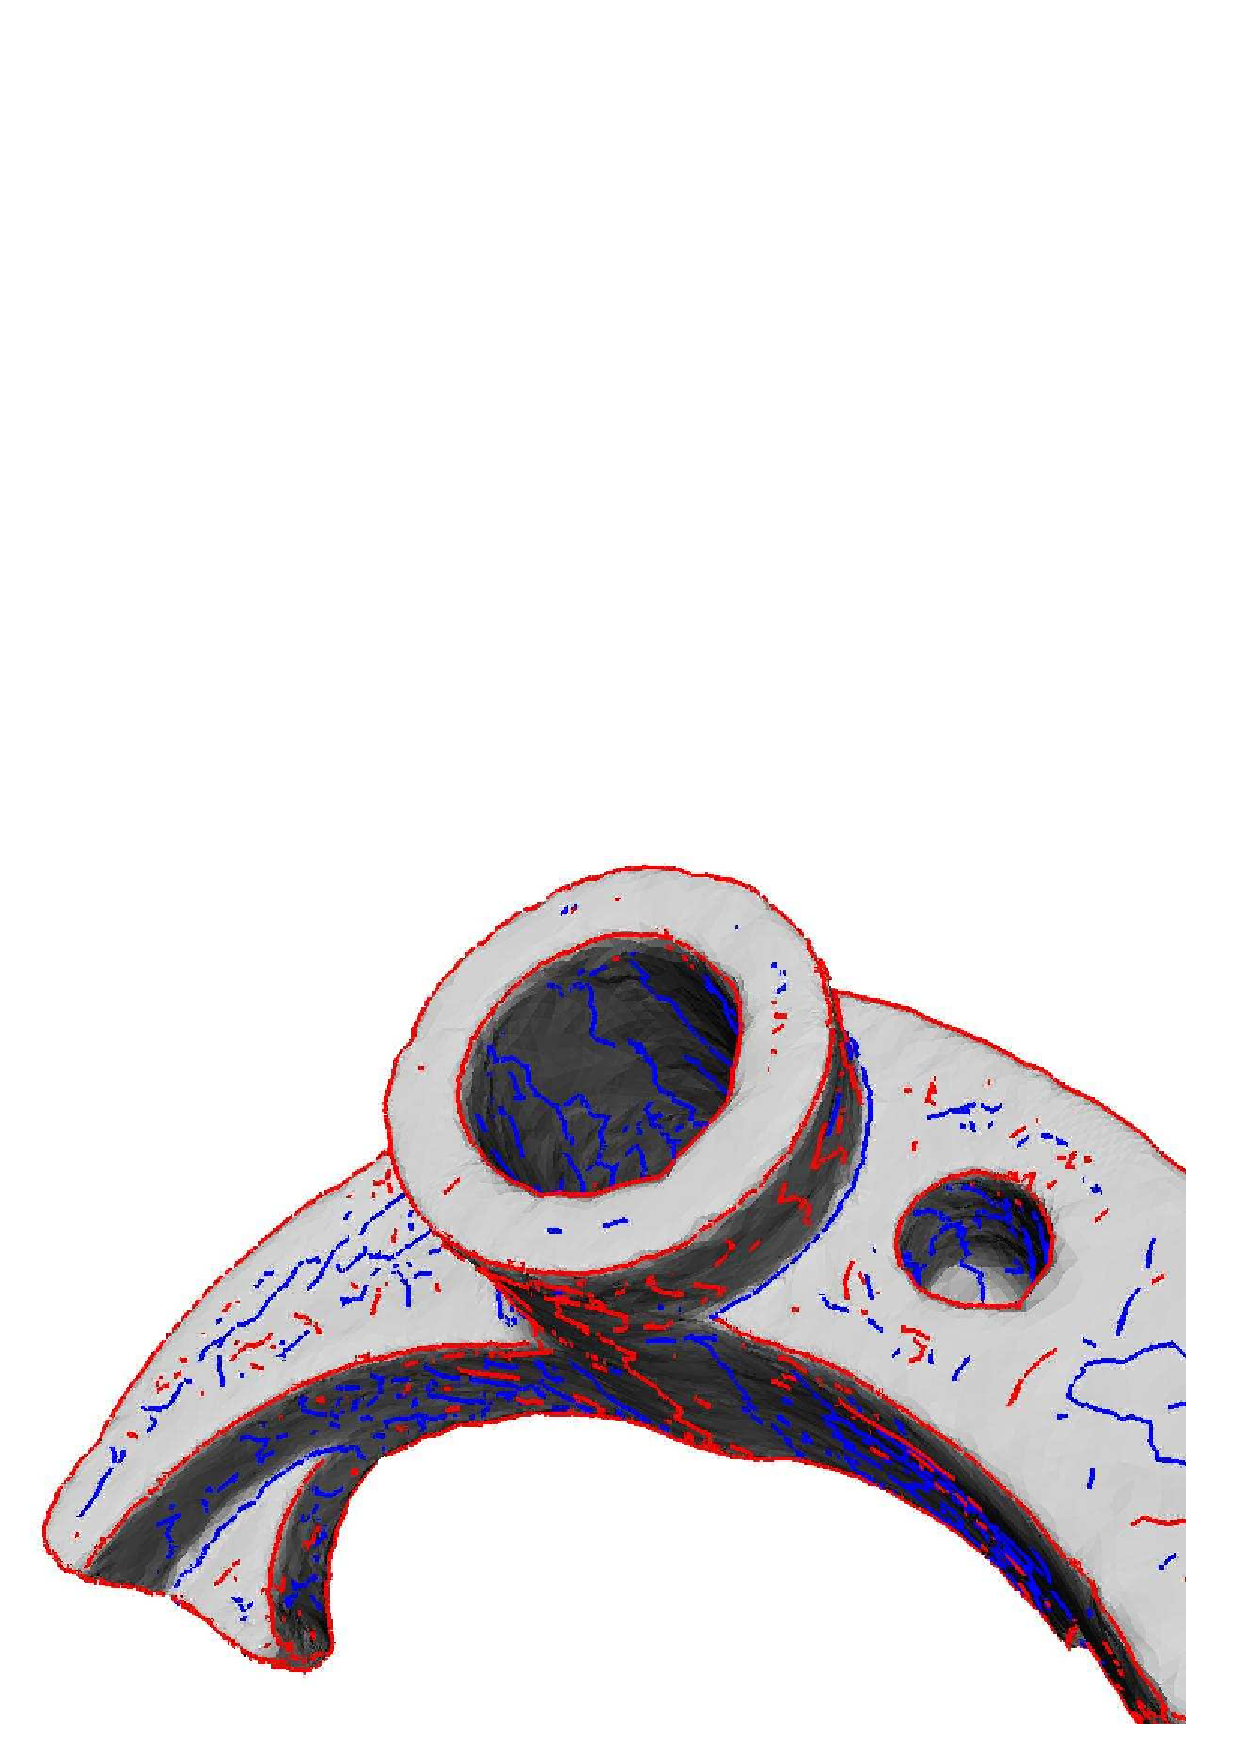
\includegraphics[width=.45\linewidth]{Ridges_3/mecanic-sub1_crest-jpg}
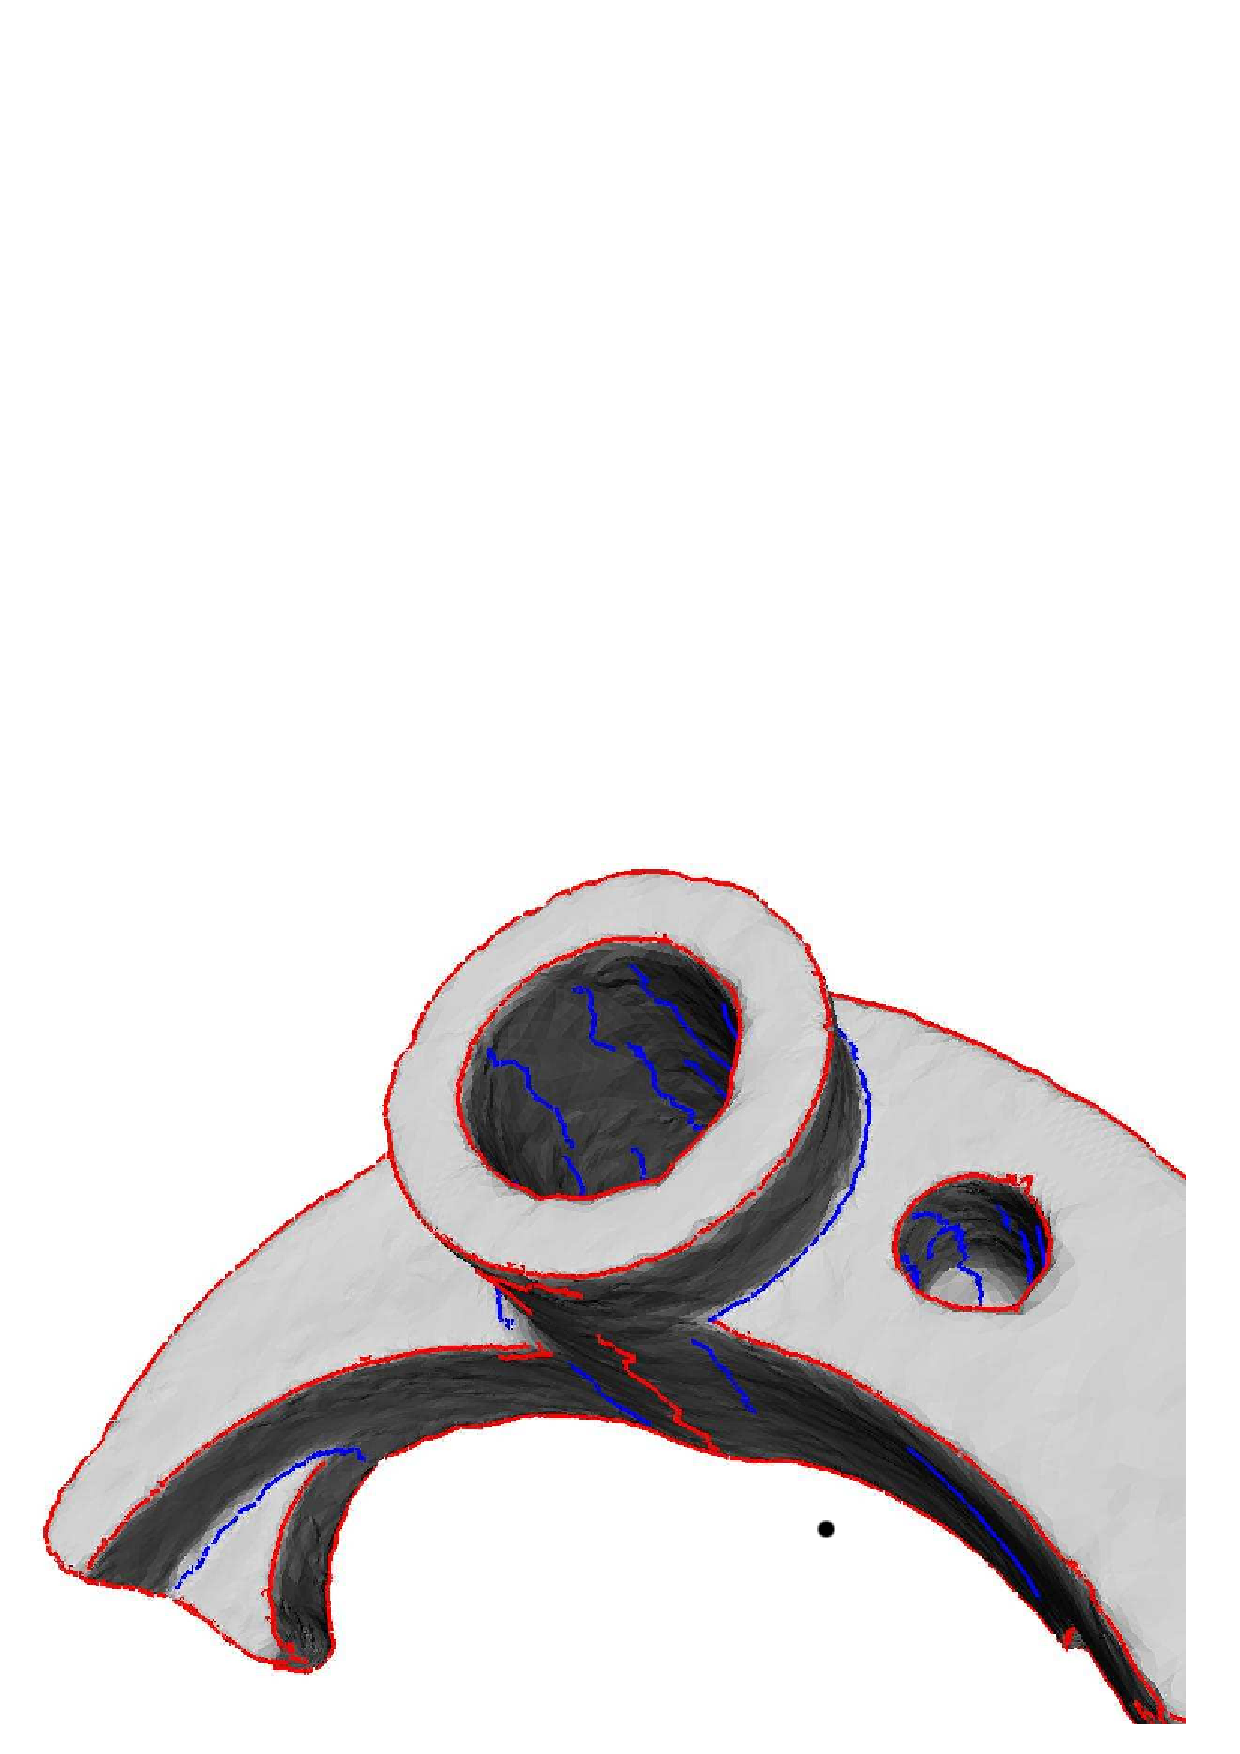
\includegraphics[width=.45\linewidth]{Ridges_3/mecanic-sub1_crestTweight1-jpg}}
\centerline{
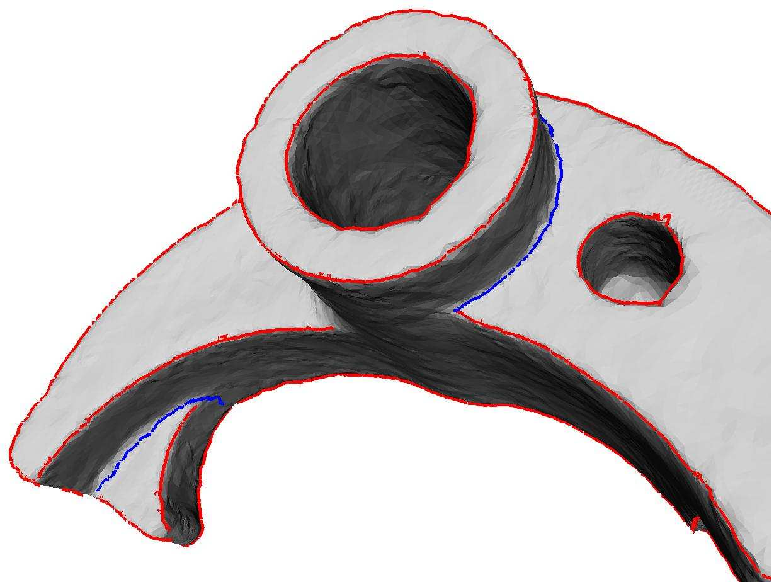
\includegraphics[width=.6\linewidth]{Ridges_3/mecanic-sub1_crestTweight1Tsharp7-jpg}}
\end{ccTexOnly}

\begin{ccHtmlOnly}
<CENTER> <img border=0 src="./mecanic-sub1_crest-jpg.png" width=200>
 <img border=0 src="./mecanic-sub1_crestTweight1-jpg.png" width=200>
</CENTER>
<CENTER>
 <img border=0 src="./mecanic-sub1_crestTweight1Tsharp7-jpg.png" width=400>
</CENTER>
\end{ccHtmlOnly}
\caption{Mechanical part (37k pts): (a) All crest lines, (b) crests filtered
with the strength threshold 1 and (c) crests filtered with the sharpness threshold 100 000.
%%
Notice that any point on a flat or cylindrical part lies on two
ridges, so that the noise observed on the top two Figs. is
unavoidable. It is however easily filtered out with the sharpness on
the bottom figure.}
\label{fig:mechanical_crest_filtered-intro} 
\end{figure} 
